\documentclass[12pt,a4paper]{article}
\usepackage[utf8]{inputenc}
\usepackage[T2A]{fontenc}
\usepackage[ukrainian]{babel}
\usepackage{fancyvrb}
\usepackage{pdflscape}

\usepackage{amsmath} % у преамбулі
\usepackage{array, multirow}
\usepackage{hyperref} % <-- Обов'язково підключіть цей пакет
\usepackage{caption}
\usepackage{booktabs}

\usepackage{xcolor}

\renewcommand{\thetable}{№\arabic{table}}
\captionsetup[table]{name=Таблиця}  % замість "Табл." буде "Таблиця"

\usepackage{graphicx} % <-- Для роботи з \includegraphics
\usepackage{geometry}
\geometry{
    left=2cm,
    right=2cm,
    top=2cm,
    bottom=2cm
}

\begin{document}

    \begin{titlepage}

        \thispagestyle{empty}
        \begin{center}
        \large
            Національний технічний університет України\\
            «Київський політехнічний інститут імені Ігоря Сікорського»\\[1em]
            Факультет інформатики та обчислювальної техніки\\
            Кафедра загальної фізики
        \end{center}

        \vfill

        \begin{center}
        \textbf{\huge Фізика}\\[2em]
        \textbf{\Large Лабораторна робота №3-10}\\[0.5em]
        «Дослід Франка-Герца» 
        \end{center}

        \vfill

        \begin{flushright}
        Виконав: студент 1 курсу ФІОТ, гр. ІО-41\\
        \textit{Давидчук А. М.}\\
        Залікова книжка № 4106\\[1em]
        Перевірив: \textit{Колган В. В.}
        \end{flushright}

        \vfill

        \begin{center}
        Київ -- 2025
        \end{center}

    \end{titlepage}

    \setlength{\parindent}{0pt}

    \textbf{\underline{Тема:}} «Дослід Франка-Герца».

    \vspace{1em}

    \textbf{\underline{Мета:}} визначення резонансного потенціалу та першого іонізаційного потенціалу атома гелію методом електронного удару.

    \vspace{1em}

    \textbf{\underline{Прилади та устаткування:}} тиратрон, блок живлення, мікроамперметр.

    \vspace{1em}

    \begin{center} \textbf{\large Теоретичні відомості} \end{center}

    \setlength{\parindent}{1.5em}

    Як відомо, саме існування атомів, а також багато їх властивостей, наприклад, лінійчатий характер спектрів випромінювання та поглинання, принципово суперечать законам класичної фізики. Коректну теорію атома дала тільки квантова механіка. Зокрема, згідно з квантовою теорією в атомі існують так звані стаціонарні або квантові стани, перебуваючи в яких атом не випромінює електромагнітної енергії. При цьому енергії стаціонарних станів утворюють дискретний набір значень 
    $E_n$, і тому при переході із стану з енергією $E_m < E_n$ атом випускає квант електромагнітного випромінювання з частотою
    $\omega_{nm}$, що визначається умовою:

    \begin{equation}
        h\omega_{nm} = E_n - E_m
        \tag{1}
    \end{equation}
    де $h = 1{,}055 \cdot 10^{-34} \text{Дж} \cdot \text{с}$ --- стала Планка.

    Класичний дослід Франка-Герца (1913 р.) демонструє дискретність енергетичного спектра
    атомів. Сутність досліду полягає B експериментальному дослідженні збудження атомів
    (у даній роботі --- гелію) у газонаповненій електронній лампі при їхніх зіткненнях прискореними електронами "електронним ударом"
    .

    На рис. 1 показано спрощену енергетичну діаграму атома гелію. У не збудженому стані атома обидва його електрони знаходяться на найнижчому енергетичному рівні
    $E_1$

    \begin{figure}[h!]

        \renewcommand{\thefigure}{\arabic{figure}} % робимо "3.1", "3.2" і т.д.

        \centering
        % Підставляєте потрібний шлях та розмір зображення:
        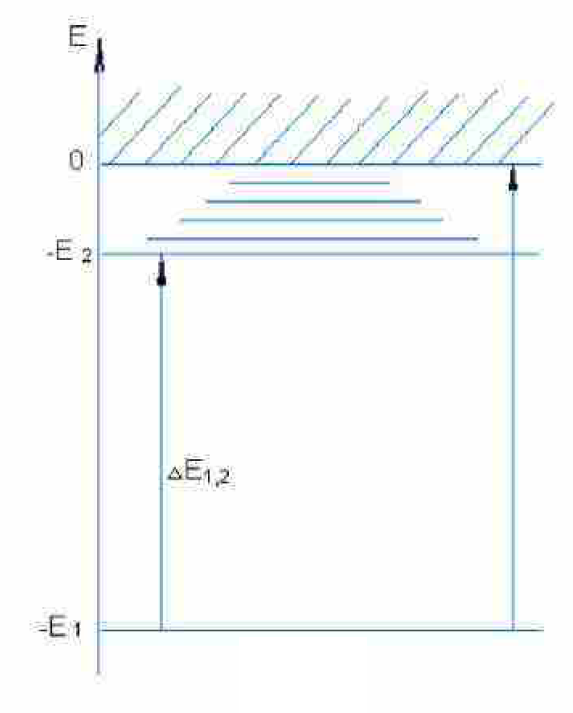
\includegraphics[width=0.3\textwidth]{1.png}
        % Підпис (зазвичай під малюнком):
        \caption{}
        % Мітка для посилань у тексті (\ref{fig:...})
        \label{fig1:schema}

    \end{figure}

    Стрілками показані переходи електронів на
    збуджений рівень $E_2$ та та в найнижчий енергетичний стан, який відповідає іонізації атома,
    $E_i$ --- енергія іонізації, тобто, мінімальна енергія, необхідна для відриву від ядра одного електрона. 

    Емітовані катодом електрони рухаються в прискорюючому полі аноду і стикаються на своєму шляху з атомами гелію. При цьому є дві можливості. 1. Якщо кінетична енергія електронів
    $E_e = eU$, набута ними у прискорюючому полі, недостатня для переведення атомів у збуджений стан 
    $\left( E_e < \Delta E_{12} \right)$, то зіткнення електронів з атомами відбуваються пружно. При цьому електрони майже не втрачають швидкості й лише змінюють напрям руху, оскільки їх маса набагато 
    (приблизно в $10^4$ разів)менша за масу атомів. 2. Друга можливість реалізується, коли електрони отримують від поля енергію, достатню для переведення атомів у збуджений або іонізований стан. У такій ситуації при зіткненнях внутрішня енергія атомів збільшується за рахунок кінетичної енергії електронів, і зіткнення стають непружними. Очевидно, що такі зіткнення можливі тільки за умови, коли 
    $E_e = eU \geq E_{12}$.
    Найменша напруга на лампі, при якій стають можливими непружні зіткнення електронів із атомами, називаються резонансним потенціалом. Резонансний потенціал визначається умовою

    \begin{equation}
        U_{\text{\textit{рез}}} = \frac{\Delta E_{21}}{e} = \frac{E_2 - E_1}{e}
        \tag{2}
    \end{equation}

    Таким чином, при напрузі на лампі $U \geq U_{\text{\textit{рез}}}$ кінетична енергія частини електронів на підльоті до анода суттєво зменшується внаслідок непружних зіткнень з атомами газу, яким заповнено лампу. 

    Ідея досліду Франка Герца, ґрунтується на тому, що такі сповільнені електрони можна затримати й не пропустити на анод, створивши біля анода невелике гальмівне поле. В такому разі поява непружних зіткнень призведе до помітного зменшення величини струму в лампі, що можна зареєструвати, вимірюючи вольт-амперну характеристику лампи, тобто, залежність анодного струму від напруги. В даній роботі визначається енергія переходу тільки в перший збуджений стан ("резонансний потенціал") і енергія однократної іонізації ("перший іонізаційний потенціал") атома гелію, оскільки визначення енергій переходу в більш високі збуджені стани пов'язане з істотним ускладненням експерименту.

    \vspace{1em}

    \begin{center} \textbf{\large Практична частина} \end{center}

    \begin{center} \textbf{Експеримент} \end{center}

    \textbf{\underline{Вимірювальна схема.}} Найпростіша принципова електрична схема установки для проведення досліду Франка-Герца показана на рис. 2 

    \begin{figure}[h!]

        \renewcommand{\thefigure}{\arabic{figure}} % робимо "3.1", "3.2" і т.д.

        \centering
        % Підставляєте потрібний шлях та розмір зображення:
        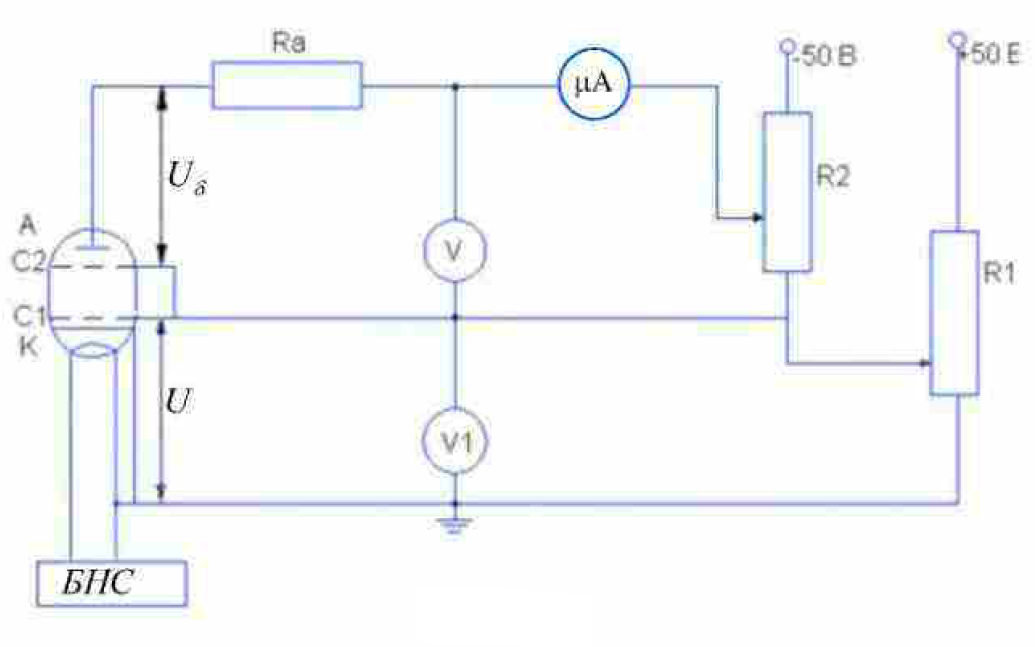
\includegraphics[width=0.5\textwidth]{2.png}
        % Підпис (зазвичай під малюнком):
        \caption{}
        % Мітка для посилань у тексті (\ref{fig:...})
        \label{fig2:schema}

    \end{figure}

    Основним елементом схеми є тиратрон
    чотирьохелектродна лампа, заповнена досліджуваним газом (гелієм) при малому тиску.
    Електроди тиратрона мають осьову симетрію: катодом слугує нитка розжарення,
    а сітки та анод мають форму коаксіальних циліндрів. Нитка розжарення живиться
    від стабілізованого джерела живлення --- БНС. Електрони, випущені катодом \textit{К}
    , потрапляють у прискорююче електричне поле між першою сіткою
    $C_1$ і катодом. Величина прискорюючої напруги $U$ регулюється потенціометром $R_1$
    і вимірюється вольтметром $V_1$.
    Тиск газу в лампі підбирається таким, аби довжина вільного пробігу електронів
    була набагато більшою, ніж відстань від катода до сітки $C_1$.
    За такої умови більша частина електронів проходить прискорююче поле
    без зіткнень з атомами і влітає в простір між сітками $C_1$ і $C_2$,
    з кінетичною енергією $W = eU$.
    У просторі між сітками, де електричного поля немає,
    відбувається зіткнення електронів з атомами. На другу сітку $C_2$,
    яка розміщена в безпосередній близькості від анода, подається потенціал,
    який на невелику величину $U$, нижчий за потенціал анода $A$.
    Тим самим у зазорі між цією сіткою та анодом для електронів створюється
    невелике гальмівне електричне поле. Затримуюча напруга $U_{\text{з}}$,
    регулюється потенціометром $R_2$ вимірюється вольтметром $V_2$.
    Анодний струм вимірюється мікроамперметром $\mu A$.

    Проаналізуємо вигляд залежності анодного струму $I$ від прискорюючої напруги
    $U$ при постійний затримуючій напрузі $U_{\text{з}}$.
    Така залежність називається вольт-амперною характеристикою (ВАХ).
    Вигляд ВАХ тиратрона показано на рис. 3.

    \begin{figure}[h!]

        \renewcommand{\thefigure}{\arabic{figure}} % робимо "3.1", "3.2" і т.д.

        \centering
        % Підставляєте потрібний шлях та розмір зображення:
        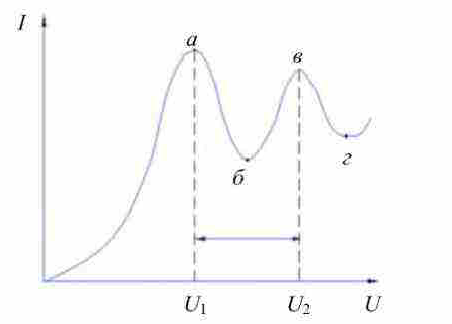
\includegraphics[width=0.5\textwidth]{3.png}
        % Підпис (зазвичай під малюнком):
        \caption{Вольт-амперна характеристика (ВАХ) тиратрона.}
        % Мітка для посилань у тексті (\ref{fig:...})
        \label{fig3:schema}

    \end{figure}
    
    При зміні прискорюючої напруги $U$ від 0 до величини
    $U_{\text{\textit{рез}}}$
    , яка визначається виразом (2), кінетична енергія електронів,
    із якою вони потрапляють в область між сітками,
    лишається недостатньою для збудження атомів.
    Через це зіткнення електронів з атомами, як відзначалося раніше, є пружними.
    При цьому змінюється тільки напрямок руху електронів, але не їхня кінетична енергія.
    Тому, з огляду на циліндричну форму анода, практично всі електрони, що проходять крізь
    сітку $C_1$, потрапляють на анод.
    Отже зіткнення електронів із атомами не впливають на анодний струм,
    і ВАХ має типовий для електронних ламп вигляд із
    збільшенням напруги $U$ струм зростає (ділянка 0 -- \textit{а} на ВАХ).
    Але коли напруга $U$ стане рівною чи трохи більшою, ніж $U_{\text{\textit{рез}}}$,
    значна частина
    електронів почне стикатися з атомами газу непружно,
    віддаючи їм майже всю кінетичну енергію.
    Відтак ці електрони виявляються нездатними подолати затримуюче поле між сіткою
    $C_2$ й анодом і не потрапляють на анод.
    Через це анодний струм різко зменшується, и на ВАХ з'являється провал (ділянка \textit{аб}).
    Але при подальшому збільшенні напруги $U$ енергія, що залишається в
    електронів після зіткнення з атомами, теж збільшується і знову стає
    достатньою для подолання затримуючого поля.
    Тому струм знову зростає, аж доки прискорююча напруга не досягне величини
    $U \geq 2U_{\text{\textit{рез}}}$ (ділянка \textit{бв} на рис. 3).
    При такій напрузі електрони отримують енергію, достатню для того, щоб
    на шляху до анода збудити два атоми.
    Відтак на ВАХ з'являється другий провал (ділянка \textit{вг} на рис. 3).

    Описану ВАХ тиратрона (рис. 3)
    можна візуально спостерігати за допомогою електронного осцилографа.
    Для цього на прискорюючу сітку $C_1$, подається змінна напруга

    \begin{equation}
        U(t) = U_0 \sin \omega t
        \tag{3}
    \end{equation}

    і така ж напруга подається на вхід $X$ осцилографа.
    В такому разі в кожен момент часу зміщення електронного променя на екрані вздовж осі
    $X$ є прямо пропорційним поданій напрузі: $Y(t) \sim U(t)$.
    З іншого боку, напруга на резисторі $R_{\text{a}}$ в анодному колі тиратрона
    (рис. 2) є прямо пропорційною до струму:
    $U_{a}(t) = I(t)R_{a}$.
    Якщо цю напругу подати на вхід $Y$ осцилографа, то зсув променя на екрані
    вздовж осі $Y$ буде прямо пропорційним силі струму в тиратроні:
    $Y(t) \sim U(t)$.
    Тому при одночасному подаванні вказаних напруг на обидва входи
    осцилографа електронний промінь буде рухатися по траєкторії,
    форма котрої співпадає з кривою $I(U)$ тобто, з вольт-амперною характеристикою.
    Оскільки напруга $U$ (вираз (4)) періодично змінюється з промисловою
    частотою $\nu = \omega / 2\pi$ = 50 Гц,
    траєкторія променя буде точно відтворюватися 50 разів за секунду,
    й на екрані осцилографа буде спостерігатися стійке зображення ВАХ.
    Параметри кривої на екрані залежать не лише від напруги та струму в тиратроні,
    а й від параметрів схеми осцилографа, тому в даній роботі осцилограф використовується
    тільки для спостереження ВАХ. Кількісні параметри ВАХ визначаються за
    допомогою включених у схему вимірювальних приладів (див. рис. 3). 

    \textbf{\underline{Визначення резонансного потенціалу.}} Резонансному потенціалові
    (2) на ВАХ відповідає напруга, при якій починається спад струму:
    $U_1 = U_{\text{\textit{рез}}}$,
    відповідно $U_2 = U_{\text{\textit{рез}}}$.
    Напруги $U_1, U_2$ в роботі вимірюються вольтметром.

    У зв'язку з цим необхідно зауважити наступне. Між катодом і сіткою $C_1$
    існує так звана контактна різниця потенціалів, тому покази вольтметра
    $U_{\text{\textit{в}}}$ відрізняються від різниці потенціалів, яку проходять електрони,
    на невідому величину $U_{\text{\textit{конт}}}$ так, що

    \begin{equation}
        U_{\text{\textit{в}}} = U + U_{\text{\textit{конт}}}
        \tag{4}
    \end{equation}
    Але цю похибку легко виключити,
    знайшовши різницю показів вольтметра, що відповідають точкам \textit{a} і \textit{в} на ВАХ (рис. 3) 

    \begin{equation}
        U_{\text{\textit{в2}}} - U_{\text{\textit{в1}}} = U_2 - U_1 \quad \Rightarrow \quad U_{\text{\textit{в2}}} - U_{\text{\textit{в1}}} = U_{\text{\textit{рез}}}
        \tag{5}
    \end{equation}

    \textbf{\underline{Визначення першого іонізаційного потенціалу.}} За
    досить великої енергії електрон при зіткненні з атомом може спричинити ударну
    іонізацію, при якій атом утрачає один свій електрон і перетворюється на
    однозарядний іон.
    Мінімальна необхідна для цього енергія $E_{i1}$
    називається \textit{енергією однократної іонізації} або \textit{першим іонізаційним потенціалом} атома.
    Вона залежить від природи атома (для гелію $E_{i1} = 24{,}6$ \textit{eВ}).

    Очевидно, що для іонізації атомів у тиратроні емітовані катодом електрони повинні
    прискорюватися сіткою $C_1$ до енергії $eU \geq E_{1l}$.
    Отже, іонізація спостерігається при напрузі на сітці $C_1, U \geq E_{i1}/e$, числове
    значення котрої дорівнює величині $E_{i1}$ вираженій в електрон-вольтах.

    Створені іони, потрапляючи на анод, дають внесок у вимірюваний анодний струм.
    Цей іонний струм можна зареєструвати, і, відтак, експериментально визначити
    перший іонізаційний потенціал гелію. Для цього треба забезпечити дві умови:
    1) виключити електронний струм, який створюється при великій прискорюючій напрузі,
    та 2) забезпечити легке потрапляння іонів на анод, оскільки
    прискорююче \textit{для електронів} поле між катодом і сіткою $C_1$
    спрямовує іони не на анод, а на катод.
    Обидві умови легко виконуються, якщо при вимірюваннях ВАХ перейти в
    "режим іонізації", збільшивши затримуючу напругу $U_{\text{\textit{з}}}$
    до значення 35 -- 40 В, яке істотно перевищує $U_{i1}$.
    При цьому між сітками й анодом створюється сильне прискорююче для іонів
    і гальмівне для електронів поле.
    В такому режимі анодний струм буде створюватися тільки іонами й залежатиме від
    прискорюючої напруги, як показано на рис. 4.

    \newpage

    \begin{figure}[ht]

        \renewcommand{\thefigure}{\arabic{figure}} % робимо "3.1", "3.2" і т.д.

        \centering
        % Підставляєте потрібний шлях та розмір зображення:
        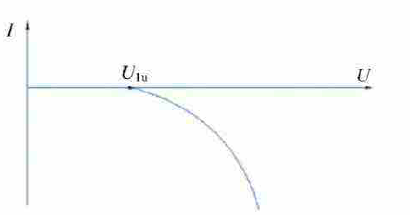
\includegraphics[width=0.5\textwidth]{4.png}
        % Підпис (зазвичай під малюнком):
        \caption{}
        % Мітка для посилань у тексті (\ref{fig:...})
        \label{fig4:schema}

    \end{figure}
    
    Тому, вимірявши прискорюючу напругу, при якій з'являється цей іонний струм, можна визначити перший іонізаційний потенціал гелію.

    \vspace{1em}

    \textbf{\textit{Примітки:}}

    \begin{enumerate}
        \item Для вимірювання анодного струму в режимі іонізації треба змінити полярність включення мікроамперметра.
        \item При визначенні $U_{i1}$ за показами вольтметра треба враховувати контактну різницю потенціалів, про яку говорилося вище.
    \end{enumerate}

    \begin{center} \textbf{Порядок виконання} \end{center}

    \begin{enumerate}
        \item Ознайомився з метою роботи та теоретичними основами процесів збудження й іонізації атомів у газі під час тліючого розряду.
        
        \item Встановив режим збудження атомів і провів серію вимірювань анодного струму при поступовому збільшенні напруги між сіткою та анодом.
        
        \item Записав експериментальні значення напруги та відповідного анодного струму в таблицю.
        
        \item Побудував вольт-амперну характеристику (ВАХ) у режимі збудження та виявив провали струму, що відповідають резонансним потенціалам.
        
        \item Визначив координати двох перших максимумів струму на ВАХ та розрахував резонансний потенціал як їхню різницю.
        
        \item За знайденим $U_{\text{\textit{рез}}}$ обчислив енергію збудження атома гелію в джоулях за формулою (2):
        \[
        U_{\text{\textit{рез}}} = \frac{\Delta E_{21}}{e} = \frac{E_2 - E_1}{e}
        \]
        
        \item Визначив контактну різницю потенціалів $U_{\text{конт}}$ на основі розбіжності між $U_{\text{рез}}$ і показами вольтметра $U_{\text{\textit{в}}}$, використовуючи формулу (3):
        \[
        U_{\text{конт}} = U_{\text{рез}} - U_{\text{\textit{в}}}
        \]
        
        \item Перейшов до режиму іонізації, змінивши полярність мікроамперметра, та провів нові вимірювання.
        
        \item Побудував ВАХ у режимі іонізації, визначив напругу зростання струму та обчислив потенціал іонізації $U_{i1}$ атома Гелію за формулою~(4):
        \[
        U_{i1} = U_{\text{\textit{в}}} - U_{\text{конт}}
        \]
        
        \item Обчислив відносне відхилення експериментального значення потенціалу іонізації від табличного значення за формулою:
        \[
        \varepsilon_{U_{i1}} = \frac{\Delta U_{i1}}{U_{theor_{i1}}} \cdot 100\%
        \]

    \end{enumerate}

    \setlength{\parindent}{0em}

    \textbf{Дані таблиць взяв із вкладених даних вимірів:}

    \setlength{\parindent}{1.5em}

    \vspace{1em}

    \noindent
    \begin{minipage}[t]{0.48\textwidth}
    \text{$U_{\text{зат}} = 7\,\text{B}$}\\[2em]
    \text{Таблиця №1}

    \vspace{0.5em}
    \begin{tabular}{|c|c|c|}
    \hline
    № & $U$, B & $I$, мкА \\
    \hline
    1. & 0 & 0 \\
    2. & 2 & 0 \\
    3. & 4 & 0 \\
    4. & 6 & 0 \\
    5. & 8 & 2 \\
    6. & 10 & 12 \\
    7. & 12 & 17 \\
    8. & 14 & 20 \\
    9. & 16 & 24 \\
    10. & 18 & 26 \\
    11. & 20 & 30 \\
    12. & 22 & 32 \\
    13. & 24 & 30 \\
    14. & 26 & 23 \\
    15. & 28 & 14 \\
    16. & 30 & 18 \\
    17. & 32 & 22 \\
    18. & 34 & 28 \\
    19. & 36 & 35 \\
    20. & 38 & 38 \\
    21. & 40 & 42 \\
    22. & 42 & 41 \\
    23. & 44 & 40 \\
    24. & 46 & 40 \\
    25. & 48 & 38 \\
    26. & 50 & 39 \\
    27. & 52 & 40 \\
    28. & 54 & 42 \\
    \hline
    \end{tabular}
    \end{minipage}
    \hfill
    \begin{minipage}[t]{0.48\textwidth}
    \text{$U_{\text{сет}} = 33\,\text{B}$}\\[2em]
    \text{Таблиця №2}

    \vspace{0.5em}
    \begin{tabular}{|c|c|c|}
    \hline
    № & $U$, B & $I$, мкА \\
    \hline
    29. & 0 & 0 \\
    30. & 2 & 0 \\
    31. & 4 & 0 \\
    32. & 6 & 0 \\
    33. & 8 & 0 \\
    34. & 10 & 0 \\
    35. & 12 & 0 \\
    36. & 14 & 0 \\
    37. & 16 & 0 \\
    38. & 18 & 0 \\
    39. & 20 & 0 \\
    40. & 22 & 0 \\
    41. & 24 & 0 \\
    42. & 26 & 0 \\
    43. & 28 & 0 \\
    44. & 30 & -2 \\
    45. & 32 & -10 \\
    46. & 34 & -14 \\
    47. & 36 & -16 \\
    48. & 38 & -17 \\
    49. & 40 & -18 \\
    50. & 42 & -20 \\
    51. & 44 & -20 \\
    52. & 46 & -22 \\
    53. & 48 & -24 \\
    54. & 50 & -26 \\
    55. & 52 & -30 \\
    56. & 54 & -33 \\
    57. & 55 & -34 \\
    \hline
    \end{tabular}
    \end{minipage}

    \newpage

    На основі даних таблиці №1 та таблиці №2 були побудовані наступні графіки:

    \begin{figure}[ht]
        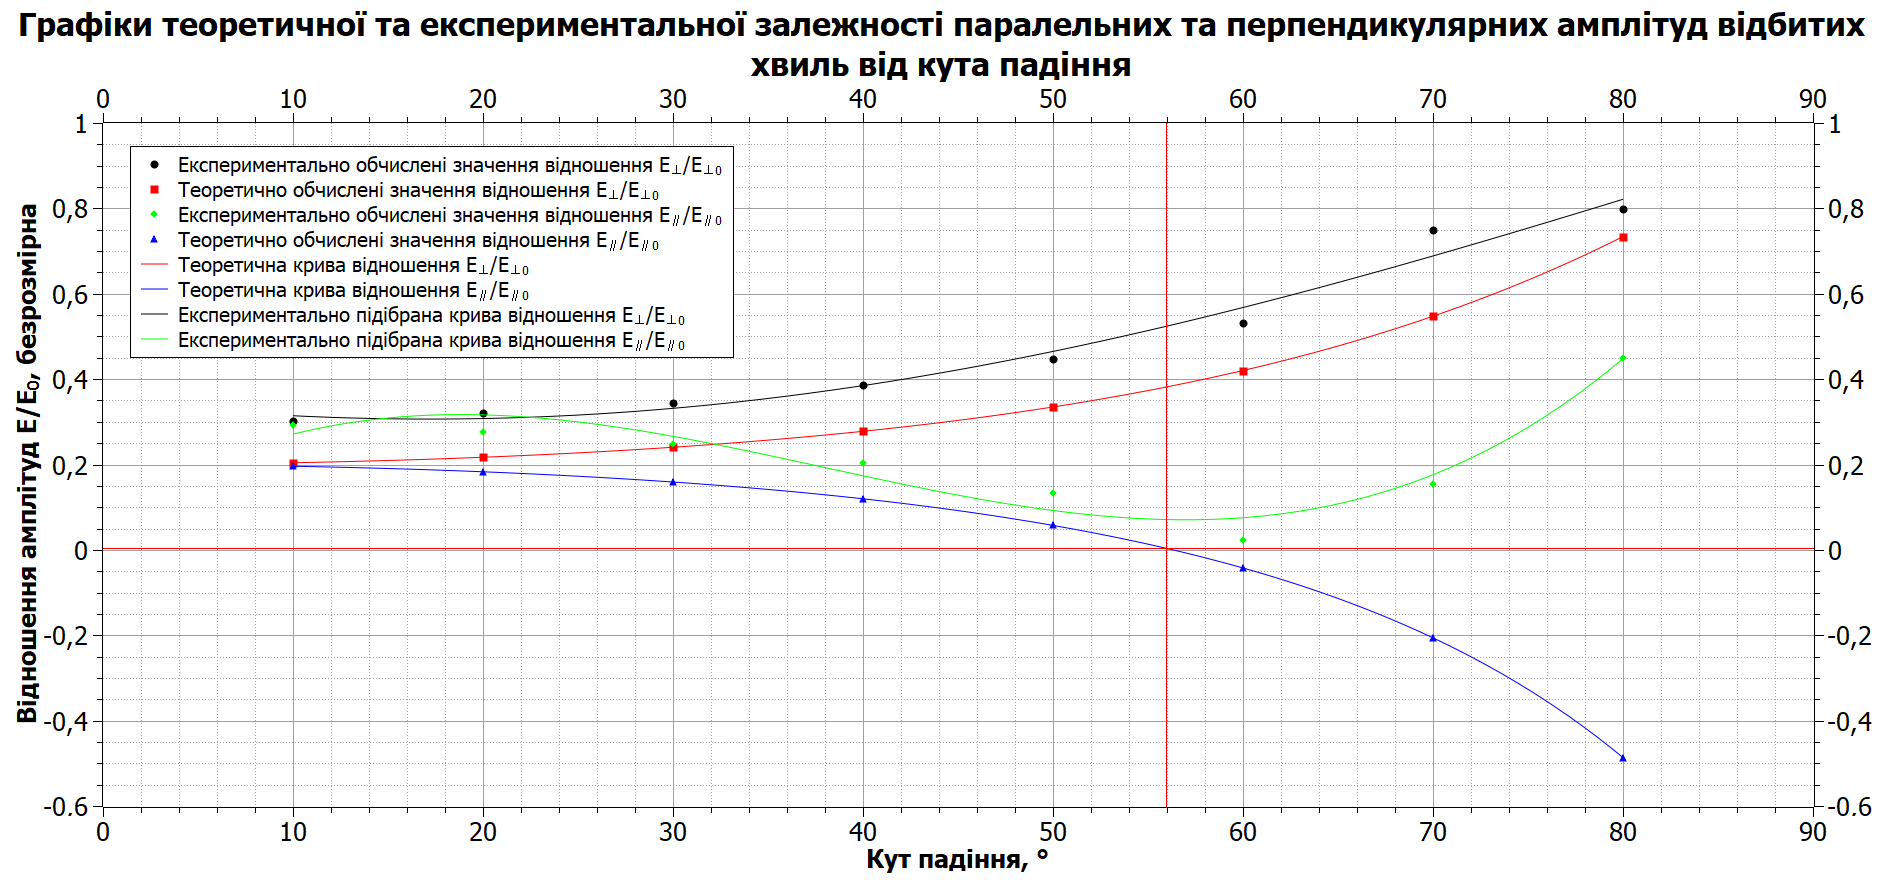
\includegraphics[width=1.0\textwidth]{graph1.png}
    \end{figure}

    \begin{figure}[ht]
        \includegraphics[width=1.0\textwidth]{graph2.png}
    \end{figure}

    Звідси визначу значення $U_{\text{\textit{з}}}$ за отриманими значеннями $U_1$ та $U_2$ з графіку 1, за формулою (5):\\[1em]
    $U_{\text{\textit{рез}}} = U_2 - U_1 = 41{,}95 - 19{,}58 = 22{,}37 $ В. Звідси можна сказати, що чисельно
    $U_{\text{\textit{рез}}}$ дорівнює енергії, поданій у еВ. Щоб подати у Джоулях, потрібно помножити $U_{\text{\textit{рез}}}$ на значення $e = 1{,}6 \cdot 10^{-19}$ Кл, тобто
    $U_{\text{\textit{рез}}} \cdot e = 22{,}37 \cdot 1{,6} \cdot 10^{-19} \approx 35{,}79 \cdot 10^{-19} $ Дж.

    Також звідси можна обчислити величину та знак контактної різниці потенціалів $U_{\text{\textit{конт}}}$, за формулою (4), приймаючи $U = U_{\text{\textit{рез}}}$, а
    також знайшовши значення $U_{\text{\textit{в}}}$ за графіком 2 ($U_{\text{\textit{в}}} \approx 25{,}94$ В). Звідси з формули (4):\\[1em]
    $U_{\text{\textit{конт}}} = U_{\text{\textit{рез}}} - U_{\text{\textit{в}}} = 22{,}37 - 25{,}94 = -3{,}57$ В.

    І щоб визначити $U_{i1}$, ми можемо знайти різницю між напругою появою іонізаційного струму та контактною напругою:\\[1em]
    $U_{i1} = U_{\text{\textit{в}}} - U_{\text{\textit{конт}}} = 25{,}94 - \left( -3{,}57 \right) = 25{,}94 + 3{,}57 = 29{,}51$ В.

    Загальновідоме теоретичне значення $U_{theor_{i1}}$ для атома Гелію з довідників приблизно дорівнює 24{,}6 В. Звідси абсолютна похибка експериментально обчисленого значення із теоретичним:\\[1em]
    $\displaystyle \varepsilon_{U_{i1}} = \frac{\Delta U_{i1}}{U_{theor_{i1}}} = \frac{\left|  U_{i1} - U_{theor_{i1}}\right|}{U_{theor_{i1}}} = 
    \frac{29{,}51 - 24{,}6}{24{,}6} = \frac{4{,}91}{24{,}6} \approx 0{,}1995$ або 19{,}95 \%.\\[2em]

    \setlength{\parindent}{0em}

    \textbf{Висновок:}

    \setlength{\parindent}{1.5em}

    У роботі досліджено вольт-амперну характеристику тліючого розряду в гелії. Визначено основні енергетичні характеристики процесу:

    \vspace{1em}

    Резонансний потенціал: \(U_{\text{рез}} = 22{,}37~\text{В}\)

    Потенціал іонізації гелію:\(U_{i1} = 29{,}51\text{В}\)

    Відносне відхилення від табличного значення \( 24{,}6~\text{В} \): \(\varepsilon \approx 19{,}95\%\)

    \vspace{1em}

    Похибка зумовлена неточністю у визначенні координат максимумів і мінімумів на експериментальній кривій, а також тим, що значення були обрані з
    апроксимуючого полінома, який має певну похибку наближення. Додатковий вплив має контактна різниця потенціалів та конструктивні особливості приладу.

    \vspace{3em}

    \begin{center} \textbf{\large Контрольні запитання} \end{center}

    \begin{enumerate}
        \item \textit{Які дослідні факти свідчать про несумісність класичної фізики пояснити будову атома?}\\[0.5em]
        Класична фізика не могла пояснити дискретність енергетичних рівнів. Дослід Френка–Герца показав, що електрони передають енергію лише при певних значеннях напруги, що суперечить класичній моделі.

        \item \textit{Які зіткнення частинок називаються абсолютно пружними, а які — непружними? Запишіть закон збереження енергії для кожного випадку.}\\[0.5em]
        Абсолютно пружні: енергія зберігається повністю.\\
        Абсолютно непружні: частина енергії йде на збудження атома.\\
        \textbf{Пружне:} $E_{\text{кін до}} = E_{\text{кін після}}$\\
        \textbf{Непружне:} $E_{\text{кін до}} = E_{\text{кін після}} + E_{\text{внутр}}$

        \item \textit{Коли в тиратрона відбуваються тільки пружні зіткнення електронів з атомами, а коли можливі й непружні?}\\[0.5em]
        Пружні — коли енергія електрона недостатня для збудження атома.\\
        Непружні — коли енергії вистачає для збудження або іонізації.

        \item \textit{Зобразіть принципову електричну схему вимірювання вольт-амперної характеристики тиратрона.}\\[0.5em]
        Катод — сітка $C_1$ — анод, з підключеними $U_1$, $U_2$ та мікроамперметром між сіткою і анодом. Джерела живлення дозволяють регулювати потенціали.

        \item \textit{Обґрунтуйте, чому крива, яка спостерігається на екрані осцилографа, відображає ВАХ тиратрона $I = f(U)$.}\\[0.5em]
        Струм $I$ змінюється відповідно до зміни напруги $U$ між сіткою й анодом, тому графік прямо показує залежність $I(U)$.

        \item \textit{Зобразіть і поясніть вигляд ВАХ тиратрона в режимі збудження атомів. Чому спостерігається другий провал на ВАХ?}\\[0.5em]
        Графік має піки й провали. Кожен провал — втрата енергії електронами при збудженні. Другий провал — результат повторного збудження.

        \item \textit{Що таке резонансний потенціал атома? Як він визначається в даному досліді?}\\[0.5em]
        Це напруга, при якій електрон передає енергію атому. Визначається як положення першого провалу струму на ВАХ.

        \item \textit{Як визначити резонансний потенціал, якщо спостерігається лише один пік? Яка при цьому можлива помилка?}\\[0.5em]
        Орієнтуються на єдиний пік. Помилка: можливо, інші піки приховані — наприклад, через обмеження напруги або невірне підключення.

        \item \textit{Як за результатами ВАХ можна визначити контактну різницю потенціалів між катодом і сіткою?}\\[0.5em]
        За формулою: $U_{\text{конт}} = U_g - U$, де $U$ — реальна напруга переходу, а $U_g$ — показ вольтметра.

        \item \textit{Що таке перший потенціал іонізації? При якій напрузі спостерігається іонізація атома?}\\[0.5em]
        Це мінімальна напруга, при якій електрон вириває електрон з атома. Спостерігається при різкому зростанні струму на ВАХ.

        \item \textit{Що потрібно зробити в експерименті, щоб перейти від режиму збудження до іонізації?}\\[0.5em]
        Потрібно підвищити напругу. У режимі іонізації струм різко зростає через лавиноподібне утворення іонів.

        \item \textit{Чому при переході в режим іонізації потрібно змінити полярність мікроамперметра?}\\[0.5em]
        Струм у ланцюзі змінює напрям. Мікроамперметр фіксує зворотний струм, тому його потрібно підключити з протилежним знаком.
    \end{enumerate}

\end{document}